%
\documentclass[12pt]{article}
%\documentclass[12pt]{memoir}
\usepackage[hyphens]{url}
\usepackage{savesym}
\usepackage{amsmath, amssymb, graphics, setspace}
\savesymbol{iint}
\usepackage{txfonts}
\restoresymbol{TXF}{iint}
\usepackage[squaren,thinqspace]{SIunits} % for units. The squaren option is REQUIRED to prevent squared def collisions
\usepackage{graphicx}                 % Packages to allow inclusion of graphics
\usepackage{color}                    % For creating coloured text and background
% Use this form with latex or pdflatex to include inline LaTeX code:
\usepackage[inline]{asymptote}
% Enable this line to support PDF hyperlinks:
%\usepackage[3D]{movie15}
\usepackage[bigfiles,noplaybutton]{media9}
% Enable this line for PDF attachments with asy environment option attach=true:
%\usepackage[dvips]{attachfile2}
%Input an asymptote preamble to define a few macros.
%%%%%%%%%
%%%%%%%%%
%%%%%%%%%
\usepackage[vmargin=1in,hmargin=1.25in]{geometry}
%\usepackage{fontspec}
\usepackage{xcolor}
\usepackage{titlesec}
%\defaultfontfeatures{Ligatures=TeX}
% Set sans serif font to Calibri
%\setsansfont{Calibri}
% Set serifed font to Cambria
%\setmainfont{Cambria}
% Define light and dark Microsoft blue colours
%\definecolor{MSBlue}{rgb}{.204,.353,.541}
%\definecolor{MSLightBlue}{rgb}{.31,.506,.741}
% Define a new fontfamily for the subsubsection font
% Don't use \fontspec directly to change the font
%\newfontfamily\subsubsectionfont[Color=MSLightBlue]{Times New Roman}
% Set formats for each heading level
%\titleformat*{\section}{\Large\bfseries\sffamily\color{MSBlue}}
%\titleformat*{\subsection}{\large\bfseries\sffamily\color{MSLightBlue}}
%\titleformat*{\subsubsection}{\itshape\subsubsectionfont}
\titleformat*{\section}{\Large\bfseries\sffamily}
\titleformat*{\subsection}{\large\bfseries\sffamily}
\titleformat*{\subsubsection}{\itshape\subsubsectionfont}

%%%%%%%%
\usepackage[colorlinks=true]{hyperref} % For creating hyperlinks in cross references
%
%\input{asy_new.pre}
%
\begin{document}
%
\begin{titlepage}
\centering
\ \\%
\vspace{3in}
{\Large \textsf{User's Manual for the AirMini Transmitter}} \\
\vspace{1.5in}

\textsf{Blueridge Engineering}\\
\url{http://blueridgeengineering.net}\\

\vspace{0.5in}
Martin Sant \\
\texttt{martan@cstone.net}\\
Darrell Lamm\\
\texttt{darrelllamm0@gmail.com}\\

\vspace{1.0in}
\today \\
\end{titlepage}
\newpage

\tableofcontents

\newpage

\section{Introduction}
The AirMini transmitter is based on the 16MHz Arduino Pro Mini and uses all open source software. 
This is an easy-to-assemble kit and gives you access (in the software) to the DCC signal so that you can manipulate it if you wish. 
The AirMini board can also be programmed to be a Receiver. 

See {\small\url{http://blueridgeengineering.net/index.php/wiki/building-the-promini-air/}} for details on hardware assembly of the AirMini kit.

You can use any DCC output (say from your Digitraxx or other DCC controller) to transmit out over the Airwire Frequencies (the channel and output power level is adjustable in the software).
This does require a small opto-isolated input-board that receives high-voltage, bi-polar DCC and converts it to unipolar, 5V DCC for input to the AirMini.

We will use some terminology that may be new to you. 
The National Model Railroad Association (NMRA) set forth a standard for communicating with decoders and other model railroad devices called ``DCC'', short for Digital Command Control.
To control and configure these devices, coded, digital voltage waveforms are sent from DCC-compliant throttles over wires (usually) to these, possibly-multiple, devices, all listening to the commands, sifting out which ones are meant for them.
These coded waveforms contain digital messages or ``packets'' that tell the recipient device what to do by means of specifying the ``Address'' of the device the command is meant for.
Most DCC packets are meant for a specific recipient, although a few kinds of messages are meant for {\em all} listening recipients.

While DCC throttles are mostly concerned with commanding the speed, direction, and other behavior of locomotives, they can also be used to reconfigure the ``decoders'' that are busy interpreting the DCC commands. 
Usually, reconfiguration involves changing lighting effects and other behavior of devices on a locomotive, and the so-called ``operations mode'' (OPS mode) or ``on-the-main'' mode is very convenient for doing so. 
Each DCC throttle manufacturer has a slightly different method for putting the throttle into ``OPS mode'', but once in this mode, they all send the same kind NRMA-compliant DCC packets to re-configure the recipient decoder, by means of changing the {\textit value} of a so-called {\textit Configuration Variable} (CV).

This last point is the source of a lot of confusion. 
A {\textit Configuration Variable} (CV) is the {\em fixed address number with a fixed purpose} where we will deliver a {\em change in its value held at this address}. 
We usually refer the {\em fixed address with a fixed purpose} as ``CV\#'', where \# is some number. 
For instance, CV1 holds the value of a device's ``short address'' (whose {\textit value} can be between 1 and 127).
The {\textit value} stored at this address can be changed, so we often refer to the {\textit value} held at the CV address \# as ``CV\#={\textit value}.


\section{AirMini Settings/Configuration}
The AirMini has a number of default configuration settings that should make it useful ``out of the box,'' and conventional DCC ``CV'' ``OPS mode'' or ``on the main'' re-programming can change these settings.

See Table~\ref{lblAirMiniSettings} for the CV's that can be changed to re-configure the Air Mini.
To change these values, the throttle the AirMini is connected to must first select the current address of the AirMini, which is 9000 by default. 
Then according the instructions for the particular throttle you are using, set the throttle in ``OPS'' or ``on-the-main'' programming of Configuration Variables (CV's).

The valid range of values for the CV's are specified in Table~\ref{lblAirMiniSettings}, so if you attempt to set an invalid value for a CV, the entry will be ignored and will NOT take effect!
All changes to CV values made in OPS mode are persistent after power-down except for CV254 (RF power level), which will reset to the original default value of 6 upon power-up.

In general, it should not be necessary to change the AirMini's address.
But, if you need to change the address, the following information will help you do so.
It's a litte complicated.
If you are not changing from a short to a long address or vice versa, no change in CV29 is needed.
The fifth bit of CV29 specifies whether a ``long'' (bit 5=1) or ``short'' (bit 5=0) address is used.
For the AirMini, no other bits of CV29 are relevant, so either set CV29=0 to use the ``short'' address specified in CV1, or set CV29=32 to use the ``long'' address specied by CV17 and CV18.

When resetting the ``long address'' for the AirMini, the user {\em must} set CV17 {\em before} setting CV18! Once the user programs the value of CV18, the AirMini's address will change to the new address, whose value is set by the funny formula:
\[\text{Address} = (\text{CV17value}-192)*256+\text{CV18value},\]
so for the default values for CV17 and CV18 in Table~\ref{lblAirMiniSettings}: (227-192)*256 + 40 = 9000.
Changing the address by first setting CV17 and then CV18 means that the AirMini will no longer accept OPS Mode changes at the {\em old} address, and the throttle's address must be changed to the {\em new} address before going back into OPS mode for any further configuration changes to the AirMini.
Similarly, if you change the value of CV29, then the address for the AirMini may be changed from long-to-short or short-to-long address, so you must accordingly change the address on the throttle to communicate with the Air Mini in OPS mode at the new address.
% We need a display with:
%  - AirMini DCC address
%  - Channel #
%  - Power level

\begin{table}
\centering
\caption{AirMini Settings and Configuration}
\label{lblAirMiniSettings}
{\small
%\begin{tabular}{|llp{40pt}p{40pt}p{100pt}|}
\begin{tabular}{|llp{40pt}lp{100pt}|}
\hline 
Feature             & CV\newline Address & Valid CV Values & Default & Comments\\
\hline
RF Channel          & CV255              & 0--16           & 0       & Airwire channels \\
RF Power$^\dagger$  & CV254              & 0--10           & 6& Experimentation is required \\
Long addr high byte & CV17               & 192--231        & 227     & Program CV17 {\em before} CV18! \\
Long addr low byte  & CV18               & 0--255          & 40      & Default CV17 \& CV18 make Address = 9000 \\
Configuration       & CV29               & 0--255          & 32      & CV29=32 to use long address \\
Short addr          & CV1                & 1--127          & 3       & CV29=0 to use short address \\
\hline
\multicolumn{5}{|l|}{$^\dagger$ Resets to default on power-up}\\
\hline
\end{tabular}
}% end of \small
\end{table}

\section{Software}

The AirMini uses open source software that can be found a \url{https://github.com/martan3d/AirMini}. 
Once the source code is down-loaded into a directory that the Arduino development environment can find, it's a snap to compile and down-load updated firmware via USB to the AirMini hardware with the Arduino Integrated Development Environment (IDE). 

Since the Pro Mini board in the AirMini does not have it's own USB plug and port to provide a connection to a PC, one end of a {\em 5V} SparkFun FTDI Basic Breakout USB connector can be attached to the six-pin connector on the Pro Mini board and the FTDI's mini USB plug connects to the PC.
Be sure to orient the FTDI plug to the Pro Mini pins correctly - match up the labeling on the plug with that of the pins on the Pro Mini board on the AirMini.
See Figures~\ref{lblFTDIUSB} and \ref{lblFTDOrientation}.

\begin{figure}
\centering
\resizebox{3 in}{!}{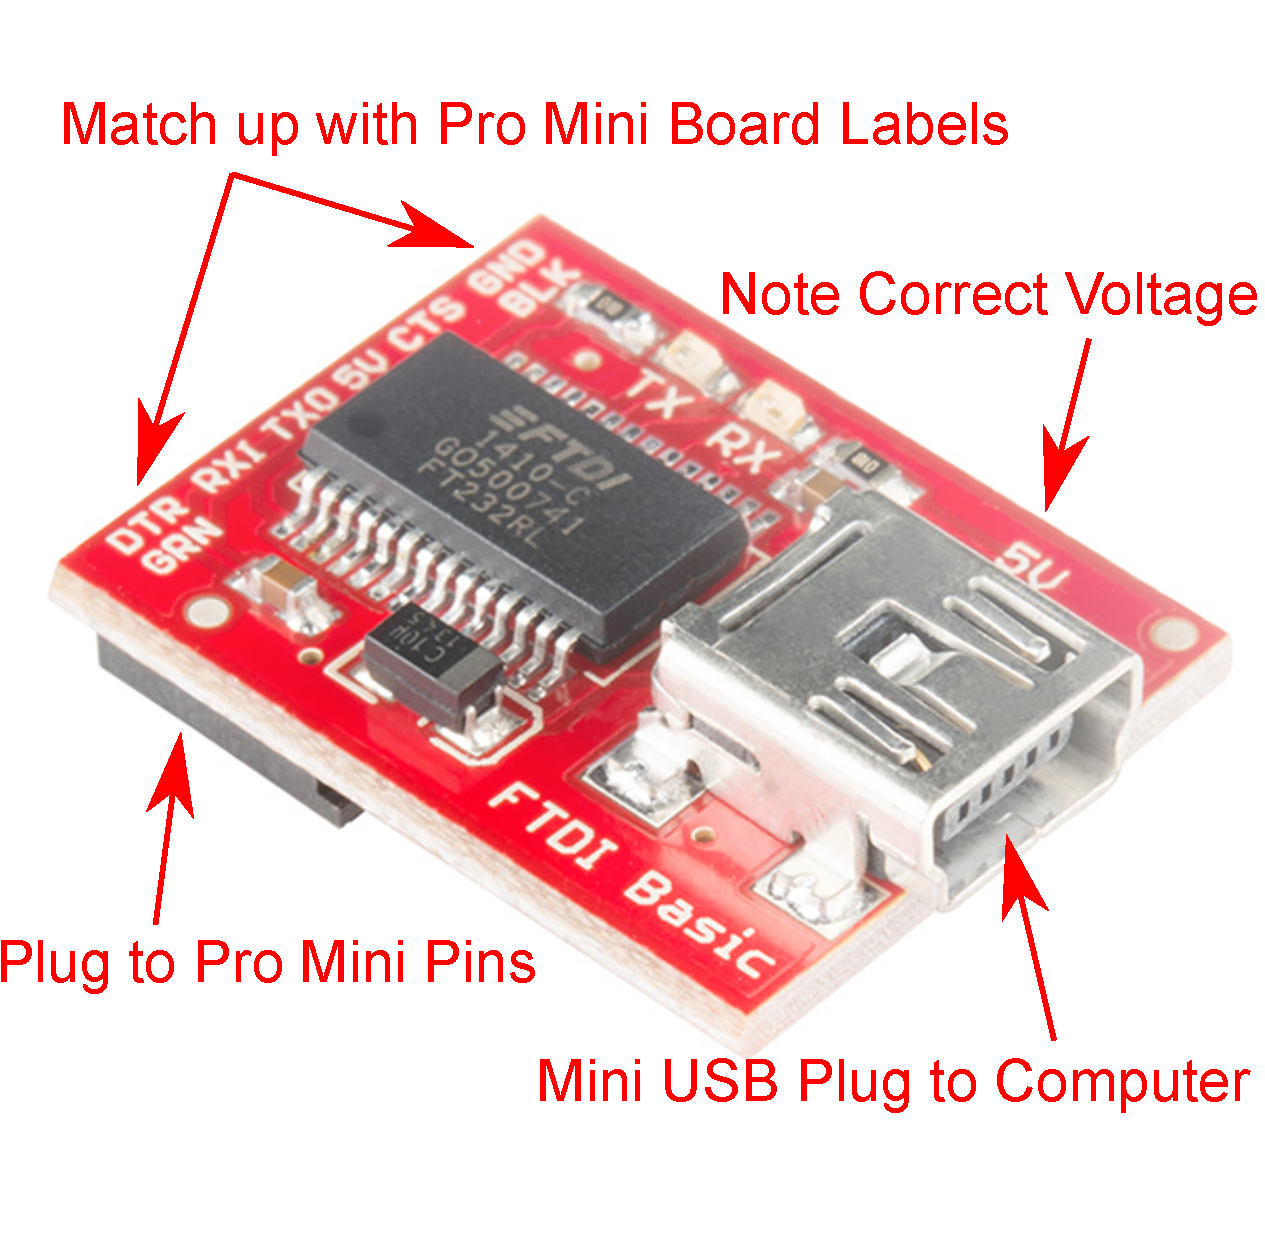
\includegraphics{FTDI_USB_Annotated.pdf}}
\caption{5V Sparkfun FTDI Basic Breakout USB connector}
\label{lblFTDIUSB}
\end{figure}

\begin{figure}
\centering
\resizebox{3 in}{!}{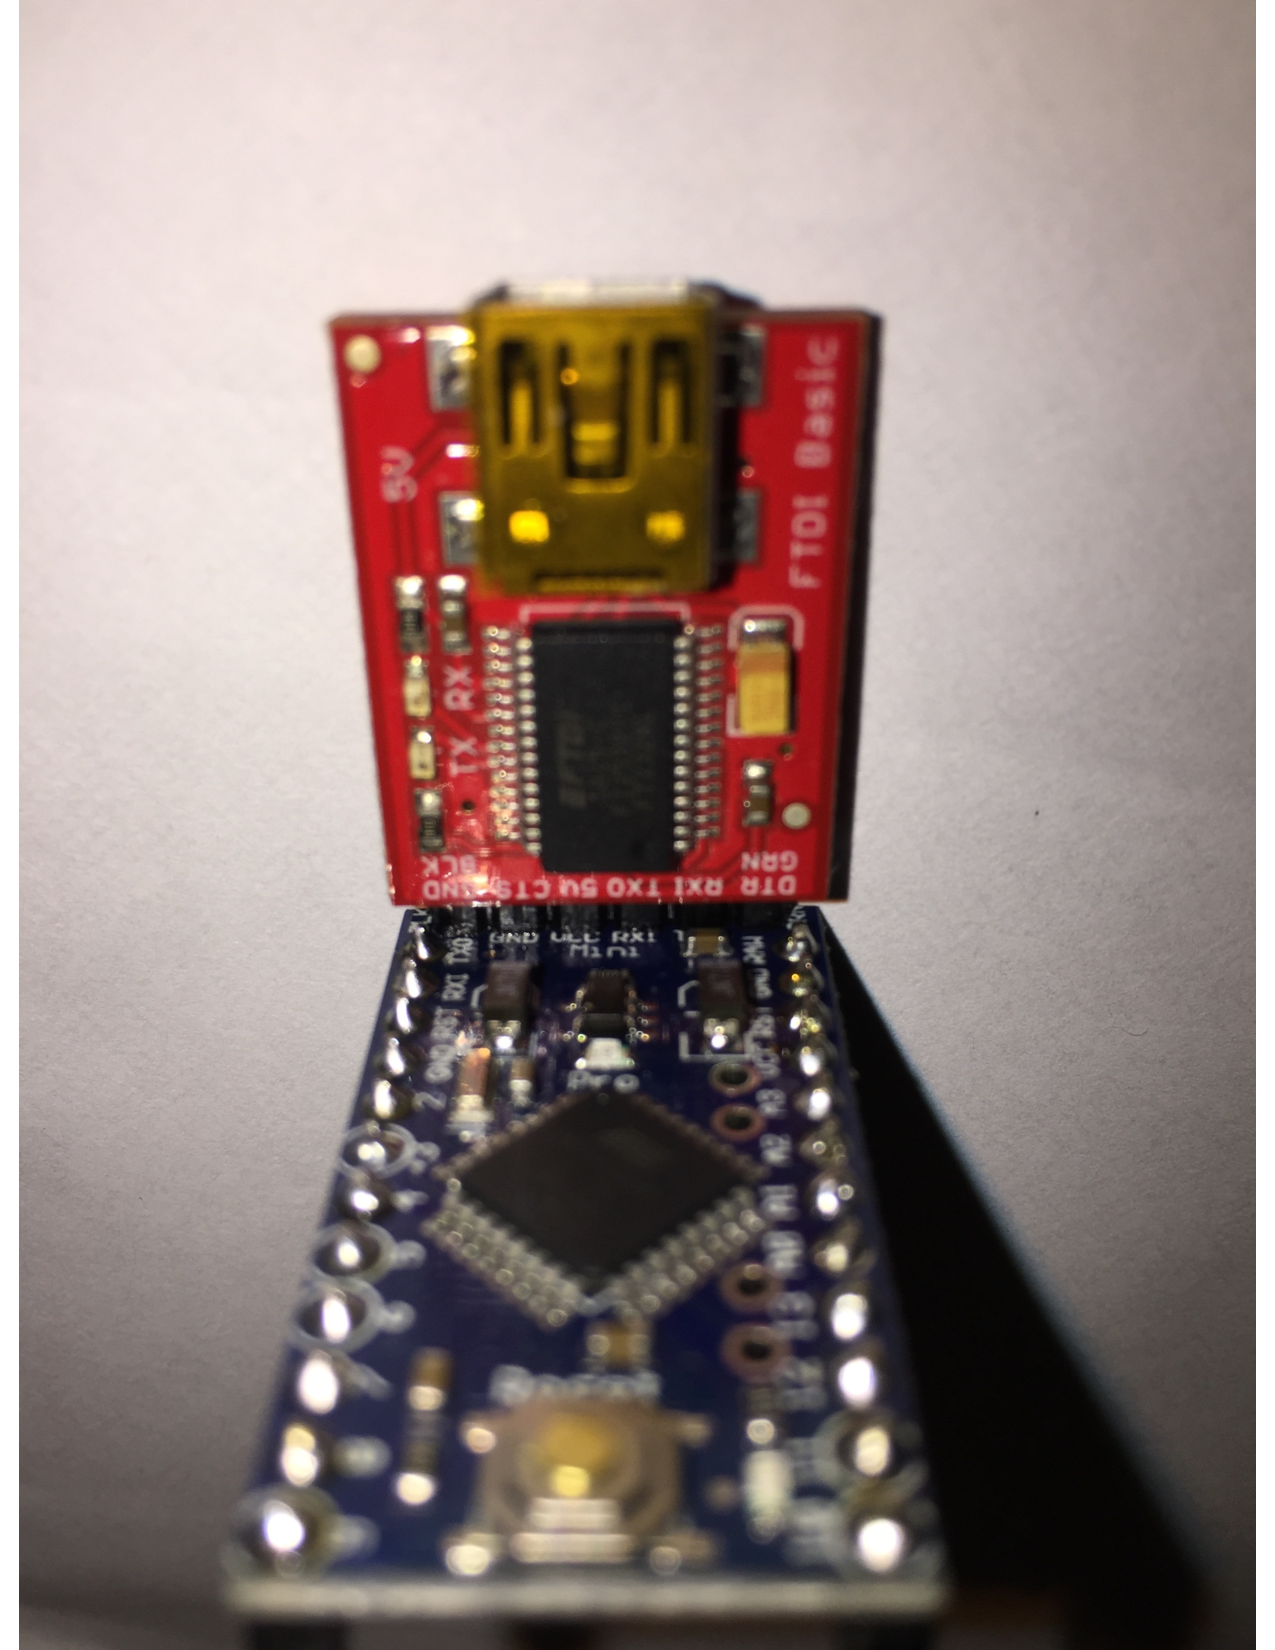
\includegraphics{FTDI_Orientation.pdf}}
\caption{Correct connection of FTDI board to Pro Mini board}
\label{lblFTDOrientation}
\end{figure}

\end{document}
